\section{实验}\label{sec:exp}

在本节中,我们对本章方法使用的数据集以及评价指标进行介绍。接下来的小节则对相关消融实验进行介绍。最后我们展示我们的实验结果并与相关文献进行对比分析。

\subsection{数据集}
我们在LM-O~\cite{Brachmann2016UncertaintyDriven6P}、YCB-V~\cite{xiang2018posecnn}和T-LESS~\cite{hodan2017t}数据集上进行实验。这些数据集涵盖了广泛的场景,包括严重遮挡、纹理缺失和具有对称的物体。LM-O数据集包含8个家用弱纹理物体。YCB-V数据集由21个物体组成,包括有纹理和无纹理的物体。T-LESS数据集为工业物体模型数据集,模型不包含模型的纹理,渲染的仿真图像也不包含真实纹理。LM-O数据集有8个不同的物体模型,每个物体约有1.2K张训练图像。相比之下,YCB-V有21个不同的物体模型,训练集更大,每个物体约有28K张图像。

由于为物体姿态标注真实数据非常耗时,我们利用BOP挑战赛~\cite{Sundermeyer2023BOPC2}提供的公开合成物理渲染(PBR)图像,证明我们的网络可以仅使用合成数据进行有效训练。
在我们的实验中,我们仅使用这些PBR图像进行训练,但使用各自数据集的真实图像进行评价。

\subsection{评价指标}

对于LM-O数据集,我们报告ADD(-S)指标,这是当代6DoF姿态估计中最常用的指标。ADD计算在使用估计姿态和使用真实姿态投影到相机坐标时,物体顶点落在距离阈值(依赖于物体大小)内的百分比。
对于对称物体,ADD(-S)的不同之处在于它匹配最近的模型点(考虑对称性)而不是完全相同的模型点。
对于YCB-V数据集,我们报告ADD(-S)的曲线下面积(AUC),最大阈值为10厘米,如文献\cite{xiang2018posecnn}所述。此外,对于这两个数据集,我们还报告BOP挑战赛定义的BOP评分指标\cite{Sundermeyer2023BOPC2}。


\subsection{消融实验}
% \begin{table}
  \centering
  \begin{tabular}{@{}c|c|c@{}}
    \toprule
     A0 &Kabsch& 86.65 \\
     A1 &RANSAC+ Kabsch& 89.12 \\
     A2 &Our Hierarchical Pruning &\textbf{89.62}\\
     \midrule
     B0 &Trust Bit Threshold 0.08& 89.55 \\
     B1 &Trust Bit Threshold 0.06& 89.61 \\
     B2 &Trust Bit Threshold 0.04& 89.59 \\
     \midrule
     C0 &Inlier Threshold: median $\rightarrow$ mean & 89.47 \\
     \midrule
     D0 & ConvNext-B~\cite{Liu2022ACF} $\rightarrow$ ResNet34~\cite{He2015DeepRL} & 88.64 \\
     \midrule
     E0 & ZebraPose(pbr)+RANSAC Kabsch&87.0\\
     E1 & ConcatRGBD+RANSAC Kabsch&84.5\\
    \bottomrule
  \end{tabular}
  \caption{Ablation study on LM-O~\cite{Brachmann2016UncertaintyDriven6P}. We conduct several ablation studies, comparing our proposed method to a RANSAC-based approach and exploring the impact of hyperparameters on the results. The results are presented in terms of average recall of ADD(-S) in \%.}
  \label{tab:ablation_study}
\end{table}
% % \vspace{-0.1cm}
\begin{table}[t]
  \centering
  \scalebox{0.78}{
  \begin{tabular}{c|c|c|c|c|c|c|c|c}
    \toprule
    Iteration Step & 1 & 2 & 3 & 4 & 5 & 6 & 7 & final \\
    \midrule
    % precision3mm(\%) & 14.3 &14.8 &16.0 &17.4 &17.6 &17.7 &17.7 &17.8\\
    precision(\%) & 66.1 &67.4 &70.3 &73.3 &73.8 &75.9 &75.9 &76.1 \\
    \bottomrule
  \end{tabular}
  }
  \caption{\textbf{Outlier removal metrics.} We evaluate precision at each iteration to validate the outlier removal process.}
  \label{tab:ourlier_removal_metrics}
  % \vspace{-0.3cm}
\end{table}


% % \vspace{-0.1cm}
% \begin{table}[t]
%   \centering
%   \scalebox{0.70}{
%   \begin{tabular}{c|c|c|c|c|c|c|c|c}
%     \toprule
%     Iteration Step & 1 & 2 & 3 & 4 & 5 & 6 & 7 & last \\
%     \hline
%     % Pre./Acc. & 14/18 &15/23 &16/31 &17/ 39&18/38 &18/39 &18/39 &18/39\\
%     precision & 0.143 &0.148 &0.160 &0.174 &0.176 &0.177 &0.177 &0.178\\
%     accuracy & 0.181 &0.226 &0.307 &0.369 &0.377 &0.385 &0.385 &0.395\\
%     \bottomrule
%   \end{tabular}
%   }
%   \label{tab:c}
% \end{table}
% % \vspace{-0.2cm}


% \begin{figure}[h]
% \begin{tikzpicture}
% \begin{axis}[
% scaled y ticks=real:1,
% ytick scale label code/.code={},
% yin = 0.10,
% ymax = 0.45,
% symbolic x coords={1, 2, 3, 4, 5, 6, 7, final},
% xtick=data,
% height=5cm,
% width=8cm,
% grid=major,
% xlabel={Iteration Step},
% ylabel={},
% y label style={at={(0.23,0.5)}},
% legend style={
%         at={(0.8,0.4)},
%         anchor=south,
%         legend columns=1,
%         nodes={scale=0.85, transform shape}
%     },
% ]
% \addplot coordinates {
% (1,0.143) 
% (2, 0.148) 
% (3, 0.160) 
% (4, 0.174) 
% (5, 0.176) 
% (6, 0.177)
% (7, 0.177)
% (final, 0.178)     
% };

% \addplot coordinates {
% (1, 0.181) 
% (2, 0.226) 
% (3, 0.307) 
% (4, 0.369) 
% (5, 0.377) 
% (6, 0.385)
% (7, 0.385)
% (final, 0.395)     
% };

% \legend{precision, accuracy}
% \end{axis}
% \end{tikzpicture}
% \vspace{-0.3cm}
%      \label{fig:rebuttal_outlier_metrics}
% \end{figure}


% the table
% % \vspace{-0.1cm}
% \begin{table}[h]
%   \centering
%   \scalebox{0.75}{
%   \begin{tabular}{c|c|c|c|c|c|c|c|c}
%     \toprule
%     Precision & 1 & 2 & 3 & 4 & 5 & 6 & 7 & last \\
%     \midrule
%     ape & 0.1835165 & 0.19163717 & 0.20734398 & 0.21708636 & 0.21839424 & 0.22571993
% & 0.22603638 & 0.22669718\\
%     can & 0.15171696& 0.15641425& 0.16956348& 0.19150146& 0.19481966 &0.20031638&
%  0.20033761& 0.20211424\\
%     cat & 0.20078315 & 0.20586396 &0.21864493 &0.23400879& 0.23796337& 0.24927481&
%  0.24941509& 0.25015868\\
%     driller & 0.18689192& 0.19229125& 0.21834646& 0.24795955& 0.25044821 &0.25428976
% & 0.25450664& 0.25564319\\
%     duck & 0.19473783 &0.19896181 &0.21088439& 0.22924452 &0.23213276 &0.23791424&
%  0.23803701& 0.23780582\\
%     eggbox & 0.06165304& 0.06344115& 0.06609498& 0.07193866 &0.07392234 &0.06026805
%  &0.06027211& 0.06115845\\
%     glue & 0.06708077 & 0.06903647& 0.07417064& 0.07652514 &0.07697378 &0.05967345&
%  0.05980055& 0.06062067\\
%     holepuncher & 0.09947989 & 0.1042863 & 0.11287402 &0.12287721 &0.12474971 &0.12981897 & 0.12994976 &0.13055156 \\
%     \hline
%     mean & 0.1432325075 &0.147741545 &0.15974035999999997 &0.17389271125 &0.17617550875000001 &0.17715944875 &0.17729439375 &0.17809372375000002\\
%     \bottomrule
%   \end{tabular}
%   }
%   \label{tab:c}
% \end{table}
% % \vspace{-0.2cm}


% \vspace{-0.1cm}
% \begin{table}[h]
%   \centering
%   \scalebox{0.75}{
%   \begin{tabular}{c|c|c|c|c|c|c|c|c}
%     \toprule
%     Accuracy & 1 & 2 & 3 & 4 & 5 & 6 & 7 & last \\
%     \midrule
%     ape & 0.22326251& 0.28157053 &0.35574974 &0.38838136& 0.39130269 &0.39988296&
%  0.40002156 &0.41002399\\
%     can & 0.1804706 & 0.21917114 &0.30355754& 0.37984198 &0.38637728 &0.39332524&
%  0.39333441 &0.40099618\\
%     cat & 0.23212725 & 0.26658097& 0.33299124& 0.38675424& 0.39587109& 0.40774114&
%  0.40780227& 0.4156004\\
%     driller& 0.21004117& 0.24263106 &0.34637324& 0.405835  & 0.40832932& 0.41159882&
%  0.41169063& 0.4185779\\
%     duck &0.2195482 & 0.25108127 &0.31921816 &0.392198 &  0.39741826 &0.40336071&
%  0.40341472& 0.41079792 \\
%     eggbox & 0.11753599 & 0.1603692&  0.21929992 &0.30882 &   0.33421371 &0.34761027
%  &0.34761211& 0.35840996\\
%     glue & 0.11509395& 0.17707283 &0.2908764 & 0.33737505& 0.3413539 & 0.34595598&
%  0.34601414 &0.36256353\\
%     holepuncher & 0.15056989& 0.20732314& 0.28882155 &0.34957936& 0.35893959 &0.3714026& 0.37145971& 0.38026054\\
%     \hline
%     mean & 0.18108119500000003 &0.22572501749999999 &0.30711097375 &0.36859812375 &0.37672573000000004 &0.385109715 &0.38516869374999996 &0.3946538025\\
%     \bottomrule
%   \end{tabular}
%   }
%   \label{tab:c}
% \end{table}
% % \vspace{-0.2cm}


% precision & 0.143 &0.148 &0.160 &0.174 &0.176 &0.177 &0.177 &0.178
% accuracy & 0.181 &0.226 &0.307 &0.369 &0.377 &0.385 &0.385 &0.395
% \begin{figure}[t]
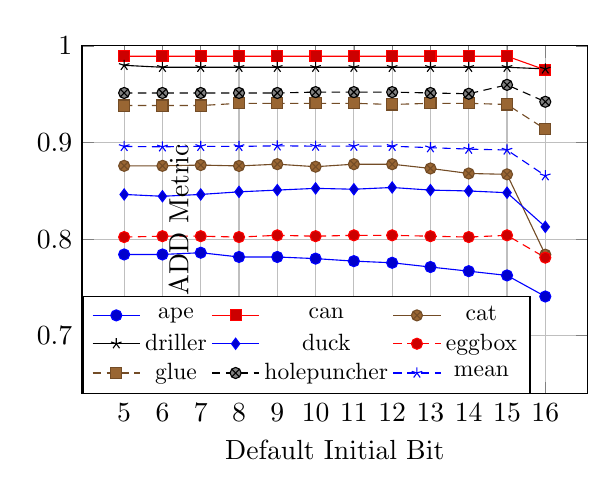
\begin{tikzpicture}
\begin{axis}[
scaled y ticks=real:100,
ytick scale label code/.code={},
ymin = 64,
ymax = 100,
symbolic x coords={5, 6, 7, 8, 9, 10, 11, 12, 13, 14, 15, 16},
xtick=data,
height=6cm,
width=8cm,
grid=major,
xlabel={Default Initial Bit},
ylabel={ADD Metric},
y label style={at={(0.23,0.5)}},
legend style={
        at={(0.445,0.0)},
        anchor=south,
        legend columns=3,
        nodes={scale=0.85, transform shape}
    },
]

\addplot coordinates {
(5,78.41) 
(6, 78.41) 
(7, 78.59) 
(8, 78.15) 
(9, 78.15) 
(10, 77.98)
(11, 77.72)
(12, 77.55)
(13, 77.11)
(14, 76.68)
(15, 76.24)
(16, 74.06)           
};


\addplot coordinates {
(5,98.92) 
(6, 98.92) 
(7, 98.92) 
(8, 98.92) 
(9, 98.92)
(10, 98.92)
(11, 98.92)
(12, 98.92)
(13, 98.92)
(14, 98.92)
(15, 98.92)
(16, 97.51)
};

\addplot coordinates {
(5,87.58) 
(6, 87.58) 
(7, 87.66) 
(8, 87.57) 
(9, 87.75)
(10, 87.49)
(11, 87.75)
(12, 87.75)
(13, 87.31)
(14, 86.79)
(15, 86.7)
(16, 78.39)
};

\addplot coordinates {
(5,97.98) 
(6, 97.78) 
(7, 97.78) 
(8, 97.78) 
(9, 97.78)
(10, 97.78)
(11, 97.78)
(12, 97.78)
(13, 97.78)
(14, 97.78)
(15, 97.78)
(16, 97.61)
};

\addplot coordinates {
(5,84.62) 
(6, 84.43) 
(7, 84.62) 
(8, 84.89) 
(9, 85.07)
(10, 85.25)
(11, 85.16)
(12, 85.34)
(13, 85.07)
(14, 84.98)
(15, 84.8)
(16, 81.27)
};

\addplot coordinates {
(5,80.21) 
(6, 80.3) 
(7, 80.3) 
(8, 80.21) 
(9, 80.39)
(10, 80.3)
(11, 80.39)
(12, 80.39)
(13, 80.3)
(14, 80.21)
(15, 80.39)
(16, 78.08)
};

\addplot coordinates {
(5,93.82) 
(6, 93.82) 
(7, 93.82) 
(8, 94.05) 
(9, 94.05)
(10, 94.05)
(11, 94.05)
(12, 93.93)
(13, 94.05)
(14, 94.05)
(15, 93.93)
(16, 91.37)
};

\addplot coordinates {
(5,95.12) 
(6, 95.12) 
(7, 95.12) 
(8, 95.12) 
(9, 95.12)
(10, 95.21)
(11, 95.21)
(12, 95.21)
(13, 95.12)
(14, 95.04)
(15, 95.96)
(16, 94.21)
};

\addplot coordinates {
(5,89.59) 
(6, 89.55) 
(7, 89.60) 
(8, 89.59) 
(9, 89.65)
(10, 89.62)
(11, 89.62)
(12, 89.61)
(13, 89.46)
(14, 89.31)
(15, 89.22)
(16, 86.56)
};

\legend{ape, can, cat, driller, duck, eggbox, glue, holepuncher, mean}
\end{axis}
\end{tikzpicture}
\vspace{-0.3cm}
     \caption{We conduct an ablation study on selecting the default initial bit $m_{default}$ using $8$ objects from the LM-O dataset.
     The flat curve illustrates that our proposed design is robust and has a clear advantage to the non-hierarchical variant ($16$ as initial bit). }
     \label{fig:ablation_initial_bit}
\end{figure}


% \begin{table}
  \centering
  \resizebox{\textwidth}{!}{%
  \begin{tabular}{c|c|c|c|c|c|c|c}
    \toprule 
    \multirow{2}{*}{方法} & \multicolumn{2}{c|}{RGB 输入方法} & \multicolumn{5}{c}{RGB-D 输入方法} \\ 
         \cline{2-8}
      & GDR-Net\cite{wang2021gdr} 
& ZebraPose\cite{su2022zebrapose}&  PR-GCN\cite{Zhou2021PRGCNAD} 
&  FFB6D\cite{he2021ffb6d} 
& RCVPose\cite{wu2022vote} 
& DFTr\cite{zhou2023deep} &本文方法\\
    \midrule
     ape & 46.8 
& 57.9& 40.2 
& 47.2 
&  60.3 
& 64.1 &  \textbf{78.0}\\
     can & 90.8 
& 95.0& 76.2 
& 85.2 
&  92.5 
& 96.1 &  \textbf{98.9}  \\
     cat & 40.5 
& 60.6& 57.0 
& 45.7 
&  50.2 
& 52.2 &  \textbf{87.5}\\
     driller & 82.6 
& 94.8& 83.2 
& 81.4 
&  78.2 
& 95.8 &  \textbf{97.8}\\
     duck & 46.9 
& 64.5& 30.0 
& 53.9 
&  52.1 
& 72.3 &  \textbf{85.3}\\
     eggbox* & 54.2 
& 70.9& 68.2 
& 70.2 
&  \textbf{81.2} 
& 75.3 &  80.3\\
     glue* & 75.8 
& 88.7& 67.0 
& 60.1 
&  72.1 
& 79.3 &  \textbf{94.1}\\
     holepuncher & 60.1 
& 83.0& \textbf{97.2} 
& 85.9 
& 75.2 
& 86.8 &  95.2  \\
     \hline
     均值 & 62.2 & 76.9&  65.0 &  66.2 &  70.2 & 77.7 & \textbf{89.6}\\
    \bottomrule
  \end{tabular}
  }
  \caption{LM-O数据集上ADD-S对比结果}
  \label{tab:lmo_results_table_}
\end{table}


% \begin{table}
  \centering
  \caption{YCB-V数据集上AUC对比结果}
  \label{tab:ycbv_results_table}
  \resizebox{0.4\textwidth}{!}{%
  \begin{tabular}{@{}l|c|c|c@{}}
    \toprule
     \multicolumn{2}{c|}{方法} & \makecell{AUC of\\ADD-S} & \makecell{AUC of\\ADD(-S)} \\
    \midrule
    \multirow{3}{*}{\rotatebox{90}{RGB}} & SO-Pose~\cite{Di_2021_ICCV} &  90.9 &  83.9  \\
     & GDR-Net~\cite{wang2021gdr} &  91.6 &  84.4 \\
     & ZebraPose~\cite{su2022zebrapose} & 90.1 & 85.3\\
     \midrule
    \multirow{5}{*}{\rotatebox{90}{RGB-D}} & PVN3D~\cite{he2020pvn3d} &  95.5 &  91.8 \\
     & RCVPose~\cite{wu2022vote} &  96.6 &  95.2 \\
     & FFB6D~\cite{he2021ffb6d} &  96.6 &  92.7 \\
     & DFTr~\cite{zhou2023deep} & 96.7 & 94.4\\
     & 本章方法 &  \textbf{97.6} &  \textbf{95.5}  \\
    \bottomrule
  \end{tabular}
  }
\end{table}

% \begin{table*}
  \centering
  \begin{tabular}{l|c|c|c|c|c|c}
    \toprule
     \textbf{Method} & Refinement & LM-O & YCB-V & T-LESS & mean & time(sec) \\
    \midrule
    FFB6D-CVPR21-PBR-NoRefinement~\cite{he2021ffb6d} &  - & 68.7 &  75.8  & - & 72.3$^*$ & 0.19$^*$\\
    RCVPose 3D\_SingleModel\_VIVO\_PBR~\cite{wu2022vote} &  ICP~\cite{Rusinkiewicz2001EfficientVO} & 72.9 &  84.3  & 70.8 & 76.0 & 1.33\\
    SurfEmb-PBR-RGBD~\cite{Haugaard2021SurfEmbDA} &  custom~\cite{Haugaard2021SurfEmbDA} & 76.0 &  79.9  & 82.8 & 79.6 & 9.04\\
    RADet+PFA-PBR-RGBD~\cite{Hai2023RigidityAwareDF} &  PFA~\cite{hu2022perspective} & 79.7 &  82.6  & 80.2 & 80.8 & 2.63\\
    GDRNPP-PBR-RGBD-MModel~\cite{liu2022gdrnpp_bop} &  $\sim$CIR~\cite{lipson2022coupled} & 77.5 &  90.6  & \textbf{85.2} & 84.4 & 6.37\\
    HiPose (ours) &  - & \textbf{79.9} &  \textbf{90.7}   & 83.3 & \textbf{84.6} & \textbf{0.16}\\
    \bottomrule
  \end{tabular}
  \caption{Comparison to leading methods of the BOP Challenge~\cite{Sundermeyer2023BOPC2} that trained on synthetic PBR data only w.r.t. BOP score.  ($\sim$) denotes similar to CIR\cite{lipson2022coupled}. $^*$ averaged over LM-O and YCB-V only as T-LESS results are not provided for this method.}
  \label{tab:bop_score_table}
\end{table*}



% \begin{table}
%   \centering
%   \begin{tabular}{@{}l|c|c|c|c}
%     \toprule
%      \makecell{Method} & LMO & YCBV & TLESS & time(sec) \\
%     \midrule
%     \small{\makecell{FFB6D-CVPR21-\\PBR-NoRefinement~\cite{he2021ffb6d}}} &  68.7 &  75.8  & - & -\\
%     \small{\makecell{GDRNPP-PBR-\\RGBD-MModel~\cite{liu2022gdrnpp_bop}}}} &  77.5 &  90.6  & \textbf{85.2} & 6.26\\
%     \small{\makecell{RCVPose 3D\_\\SingleModel\_VIVO\_PBR~\cite{Wu2021VoteFT}}}} &  72.9 &  84.3  & 70.8 & 1.33\\
%     \small{\makecell{RADet+PFA-\\PBR-RGBD~\cite{Hai2023RigidityAwareDF}}}} &  79.7 &  82.6  & 80.2 & 2.63\\
%     \small{\makecell{SurfEmb-PBR-\\RGBD~\cite{Haugaard2021SurfEmbDA}}}} &  76.0 &  79.9  & 82.8 & 9.04\\
%     \small{\makecell{HiPose (ours)} &  \textbf{79.9} &  \textbf{90.7}}   & 83.3 & \textbf{0.14}\\
%     \bottomrule
%   \end{tabular}
%   \caption{\textbf{Comparison with Leaders on BOP Challenge~\cite{Sundermeyer2023BOPC2}}. We compare our ZebraPose with state of the art w.r.t AUC of ADD(-S) and AUC of ADD-S in \%. (-) denotes results missing from the original paper.}
%   \label{tab:bop_score_table}
% \end{table}

% In the following, we perform several ablation studies with the LM-O dataset. We summarize the results in \autoref{tab:ablation_study}, \autoref{tab:ourlier_removal_metrics} and  \autoref{fig:ablation_initial_bit}.

% \textbf{Effectiveness of Correspondence Pruning.}
% We first focus on the effectiveness of our proposed hierarchical correspondence pruning.  
% In the experiment (A0) in \autoref{tab:ablation_study}, we directly solve the object pose with the Kabsch Algorithm. The promising results highlight the effectiveness of the binary encoding. However, compared to our other experiments reveals that the predicted correspondences from the network are still noisy and contain outliers. 

% Comparing A1 with A0, the most common method for identifying outliers using RANSAC framework, we observed a $2.47\%$ recall improvement. The results of A1 heavily depend on the choice of hyper-parameters, including the number of correspondences used in each iteration, the number of RANSAC iterations, and the inlier threshold in each iteration. Additionally, random seed variations can also impact the results. In this experiment, we utilized the public RANSAC and Kabsch algorithm from Open3D~\cite{zhou2018open3d}. Note that we explored multiple parameter combinations and reported the best results among them.

% In contrast to the RANSAC scheme, our hierarchical correspondence pruning provides stable results analytically, irrespective of the random seed. 
% In experiment A2, we chose the $10_\text{th}$ bit as our initial bit and defined the confidence bit based on predicted logits higher than $0.52$ or lower than $0.48$. As shown in \autoref{tab:ablation_study}, compared to not using any outlier strategy (A0), our approach (A2)  improves recall by about $3\%$ while outperforming the best results achievable by RANSAC. 

% We also estimate the precision metrics of outlier removal at each iteration in \autoref{tab:ourlier_removal_metrics}. A true sample is defined when the distance between estimated coordinates and ground truth fall under a 10mm threshold. The increase in precision confirms the gradual removal of low-quality correspondences. In the following ablation studies, we demonstrate that our approach is also robust to the choice of hyper-parameters.

% \textbf{Influence of Default Initial Bit.} Using smaller initial bits implies matching the point to a relatively coarse surface correspondence. However, our trust-bit-based initial surface selection ensures that each vertex is considered separately and corresponds to its most reliable initial bit.

% As demonstrated in \autoref{fig:ablation_initial_bit}, our proposed design is robust to the choice of initial bit from $5_\text{th}$ bit to $11_\text{th}$ bit. %For some objects, we observe a performance drop when the initial bit $m$ is greater than $11$, as too few iterations are not sufficient to locate all outliers. 
% We observe some performance drops when we start from the $12_\text{th}$ bit, and a significant drop when directly using $16_\text{th}$ bit, underscoring the importance of our hierarchical correspondence pruning. By calculating the mean recall across all 8 objects, we noticed that using the $9_\text{th}$ to $11_\text{th}$ bits as the initial bit provides slightly higher results. Considering both accuracy and computational efficiency, we consistently use the $10_\text{th}$ bit as our default initial bit.


% \textbf{Threshold for the Trust Bit.}
% The initial bit for each point and our inlier identification strategy is closely tied to the choice of the trust bit. By varying the threshold $0.02$ used in experiment A2 (predicted logits greater than 0.52 or smaller than 0.48), we alter the trust bit threshold in experiments B0, B1, and B2. As indicated by the experimental results, when the threshold is greater than $0.08$, we start to observe a small performance drop. Overall, the results remain quite stable within the threshold range of $0.02$ to $0.08$. This demonstrates the relative robustness of our approach to the choice of the trust bit.

% \textbf{Criteria used in Correspondence Pruning.}
% The default criterion for distinguishing inliers and outliers in correspondence pruning is based on the median of distance $l$ defined in Equation~\ref{eq:l}. We replaced the median criterion for the inlier threshold used in A2 with a mean criterion in C0, resulting in a decrease in average recall. It is comprehensible that utilizing indicators associated with the median produces superior outcomes, given the median's ability to disregard the impact of extreme values.

% \textbf{Effectiveness of CNN Backbone.}
% To ensure comparability with recent research employing the transformer architecture and ConvNext~\cite{Liu2022ACF} feature backbone, we default to using ConvNext as our image feature extraction network. Additionally, we provide results of experiment (D0) in \autoref{tab:ablation_study} using ResNet as the feature backbone to offer further insights for comparison with earlier approaches. Results show that the choice of feature backbone only has a marginal effect. 

% \textbf{Naive RGB-D baselines.}
% Using the networks provided by ZebraPose, we back-project 2D pixels into 3D points using the depth map, followed by pose estimation using RANSAC + Kabsch for 3D-3D correspondence(E0). We also implement "Concat"(E1), a naive baseline model that learns 2D-3D correspondence, yet solves the pose with 3D-3D correspondences. In the "Concat" baseline, we concatenate the RGB and depth channels as input for the CNN. However, the absence of a pretrained CNN model appears to make the results worse. Nonetheless, none of the baselines surpass HiPose, suggesting that direct learning of 3D-3D correspondences is more effective.

% \subsection{Comparison to State of the Art}
% In the following, we compare HiPose to the state of the art using various metrics on multiple datasets.

% \textbf{Results on LM-O.} In \autoref{tab:lmo_results_table_}, we compare our HiPose with the state-of-the-art methods on the LM-O dataset w.r.t. the ADD(-S) score. We used the 2D detection provided by CDPN~\cite{li2019cdpn}, which is based on the FCOS~\cite{Tian2019FCOSFC} detector and trained only with PBR images provided by the BOP challenge. According to the results, HiPose outperforms all other methods by a large margin of $11.9\%$ compared to the best RGB-D method DFTr and $12.7\%$ compared to the best RGB-only method ZebraPose.

% \textbf{Results on YCB-V.} In \autoref{tab:ycbv_results_table}, we compare HiPose with the state-of-the-art methods on the YCB-V dataset w.r.t. the AUC of ADD-S and ADD(-S) score. All other methods used real and synthetic images in the training. To ensure a fair comparison, the 2D FCOS detections employed here are trained with both real and synthetic images. According to the results, HiPose again excels beyond all other methods with a significant margin (around $1\%$) when taking into account that scores on YCB-V are already close to saturation.

% \textbf{Results on the BOP Benchmark.} The BOP benchmark provides a fairer ground for comparisons, offering uniform training datasets and 2D detections for all participating methods and more informative evaluation metrics~\cite{hodan2018bop}. We used the default detections provided for the BOP Challenge 2023.

% Most methods in \autoref{tab:bop_score_table} rely on a time-consuming pose refinement step, while HiPose estimates accurate object pose directly without any pose refinement. HiPose surpasses the state-of-the-art on LM-O, YCB-V datasets and achieves a very comparable result on the T-LESS dataset. When considering the average recall across the three datasets, HiPose exhibits higher recall compared to all other methods.

% GDRNPP~\cite{liu2022gdrnpp_bop} has the most closely aligned results with HiPose, yet HiPose is approximately $\mathbf{40}$ times faster than GDRNPP with refinement. This demonstrates that HiPose is both accurate and computationally efficient.

% \subsection{Runtime Analysis}
% The inference time mainly comprises two components: 1) object detection and 2) object pose estimation. For a fair comparison, we use the same method to calculate inference speed as GDRNPP on an RTX3090 GPU. Our average object pose estimation time across the LM-O, YCB-V, and T-LESS datasets is $0.075$ seconds per image. The average 2D detection time with YOLOX~\cite{Ge2021YOLOXEY} on those three datasets is $0.081$ seconds. The fast object pose estimation time ensures the real-time applicability of our approach, especially since the costly refinement methods are not necessary.